\documentclass[english,notitlepage]{revtex4-1}  % defines the basic parameters of the document
%For preview: skriv i terminal: latexmk -pdf -pvc filnavn



% if you want a single-column, remove reprint

% allows special characters (including æøå)
\usepackage[mathletters]{ucs}
\usepackage[utf8x]{inputenc}
%\usepackage[english]{babel}

%% note that you may need to download some of these packages manually, it depends on your setup.
%% I recommend downloading TeXMaker, because it includes a large library of the most common packages.

\usepackage{physics,amssymb}  % mathematical symbols (physics imports amsmath)
\usepackage{amsmath}
\usepackage{graphicx}         % include graphics such as plots
\usepackage{xcolor}           % set colors
\usepackage{hyperref}         % automagic cross-referencing (this is GODLIKE)
\usepackage{cleveref}
\usepackage{listings}         % display code
\usepackage{subfigure}        % imports a lot of cool and useful figure commands
\usepackage{float}
%\usepackage[section]{placeins}
\usepackage{algorithm}
\usepackage[noend]{algpseudocode}
\usepackage{subfigure}
\newcommand{\imp}{\hspace{5pt}\Rightarrow\hspace{5pt}}
\newcommand\numberthis{\addtocounter{equation}{1}\tag{\theequation}}
% defines the color of hyperref objects
% Blending two colors:  blue!80!black  =  80% blue and 20% black
\hypersetup{ % this is just my personal choice, feel free to change things
    colorlinks,
    linkcolor={red!50!black},
    citecolor={blue!50!black},
    urlcolor={blue!80!black}}

%% Defines the style of the programming listing
%% This is actually my personal template, go ahead and change stuff if you want

\usepackage{listings}
\usepackage{xcolor}

\definecolor{codegreen}{rgb}{0,0.6,0}
\definecolor{codegray}{rgb}{0.5,0.5,0.5}
\definecolor{codepurple}{rgb}{0.58,0,0.82}
\definecolor{backcolour}{rgb}{0.95,0.95,0.92}

\lstdefinestyle{mystyle}{
    backgroundcolor=\color{backcolour},   
    commentstyle=\color{codegreen},
    keywordstyle=\color{magenta},
    numberstyle=\tiny\color{codegray},
    stringstyle=\color{codepurple},
    basicstyle=\ttfamily\footnotesize,
    breakatwhitespace=false,         
    breaklines=true,                 
    captionpos=b,                    
    keepspaces=true,                 
    numbers=left,                    
    numbersep=5pt,                  
    showspaces=false,                
    showstringspaces=false,
    showtabs=false,                  
    tabsize=2
}

\lstset{style=mystyle}



%% USEFUL LINKS:
%%
%%   UiO LaTeX guides:        https://www.mn.uio.no/ifi/tjenester/it/hjelp/latex/
%%   mathematics:             https://en.wikibooks.org/wiki/LaTeX/Mathematics

%%   PHYSICS !                https://mirror.hmc.edu/ctan/macros/latex/contrib/physics/physics.pdf

%%   the basics of Tikz:       https://en.wikibooks.org/wiki/LaTeX/PGF/Tikz
%%   all the colors!:          https://en.wikibooks.org/wiki/LaTeX/Colors
%%   how to draw tables:       https://en.wikibooks.org/wiki/LaTeX/Tables
%%   code listing styles:      https://en.wikibooks.org/wiki/LaTeX/Source_Code_Listings
%%   \includegraphics          https://en.wikibooks.org/wiki/LaTeX/Importing_Graphics
%%   learn more about figures  https://en.wikibooks.org/wiki/LaTeX/Floats,_Figures_and_Captions
%%   automagic bibliography:   https://en.wikibooks.org/wiki/LaTeX/Bibliography_Management  (this one is kinda difficult the first time)
%%   REVTeX Guide:             http://www.physics.csbsju.edu/370/papers/Journal_Style_Manuals/auguide4-1.pdf
%%
%%   (this document is of class "revtex4-1", the REVTeX Guide explains how the class works)


%% CREATING THE .pdf FILE USING LINUX IN THE TERMINAL
%%
%% [terminal]$ pdflatex template.tex
%%
%% Run the command twice, always.
%% If you want to use \footnote, you need to run these commands (IN THIS SPECIFIC ORDER)
%%
%% [terminal]$ pdflatex template.tex
%% [terminal]$ bibtex template
%% [terminal]$ pdflatex template.tex
%% [terminal]$ pdflatex template.tex
%%
%% Don't ask me why, I don't know.

\begin{document}

\title{\textbf{FYS3150 - Project 1}}
\author{Andrew Quan, Oskar Idland, Hishem Kløvnes, Håvard Skåli}
\date{\today}                             % self-explanatory
\noaffiliation      


% ignore this, but keep it.


\maketitle 
    
\href{https://github.com/Oskar-Idland/FYS3150-ComputationalPhysic}{GitHub Repository}
    
\section*{Problem 1}
We have the one-dimensional Poisson equation
\begin{equation}
    -\frac{\text{d}^2 u}{\text{d}x^2} = 100e^{-10x}, \hspace{15pt} x \in [0,1] \label{poisson}
\end{equation}
where the right hand side of the equation is the source term $f(x)$. We have the boundary conditions $u(0) = 0$ and $u(1) = 0$. Integrating both sides of \eqref{poisson} with respect to $x$ twice we get
\begin{align*}
    \frac{\text{d}^2 u}{\text{d}x^2} &= -100e^{-10x} \\
    \iint \left( \frac{\text{d}^2 u}{\text{d}x^2} \right) \text{d}x^2 &= -100\iint e^{-10x} \text{d}x^2 \\
    \int \left( \frac{\text{d}u}{\text{d}x}\right) \text{d}x &= -100\int \left(-\frac{1}{10}e^{-10x} + C\right)\text{d}x \\
    u(x) &= -100\left(\frac{1}{100}e^{-10x} + Cx + D\right) \\
    u(x) &= Cx + D - e^{-10x} \numberthis \label{general sol}
\end{align*}
Where $C$ and $D$ are some arbitrary constants. Invoking the boundary conditions we get
\begin{align*}
    u(0) = D - 1 = 0 &\imp D = 1 \\
    u(1) = C + 1 - e^{-10} = 0 &\imp C = e^{-10} - 1
\end{align*}
Thus, plugging these constants into the general solution and rearranging the terms, the final solution becomes
\begin{equation}
    u(x) = 1 - x\left(1 - e^{-10}\right) - e^{-10x} \label{final sol}
\end{equation}
just like we wanted to show.


\section*{Problem 2}
After creating a program that defines a vector of $x$-values between 1 and 100 and evaluates the exact solution $u(x)$ defined as in \cref{final sol}, we wrote these numbers with four decimals into a text file and plotted them against each other in Python. The resulting plot is shown in \cref{plot_problem2}.
\begin{figure}[h!]
    \centering 
    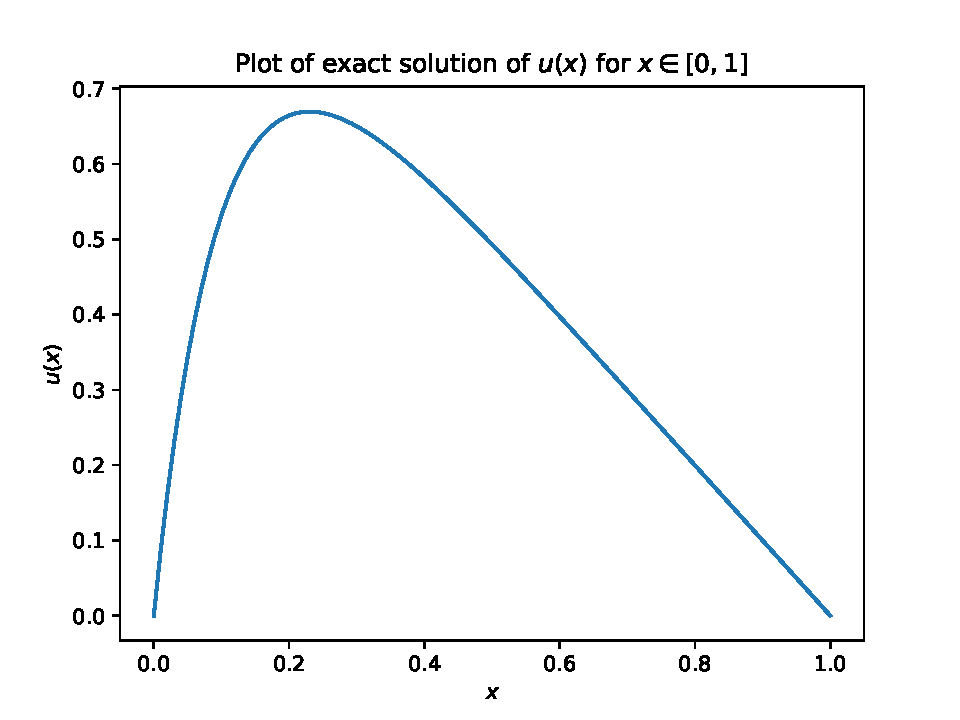
\includegraphics[scale=0.80]{../data/exactSolution.pdf} %Imports the figure.
    \caption{Plot of the exact solution of $u(x)$ for $x ∈ [0,1]$. We used 100 data points for the plot.}
    \label{plot_problem2}
\end{figure}


\section*{Problem 3}
Our aim is to derive a discretized version of the Poisson equation which lets us calculate approximates values $v$ of the exact values $u$. To create this program we need to discretize the double derivative, which we can do by recalling its definition:
\begin{equation}
    \frac{\text{d}^2u}{\text{d}u^2} = \lim_{\text{d}x\to 0}\frac{-u(x -\text{d}x) + 2u(x) - u(x + \text{d}x)}{\text{d}x^2} 
\end{equation}
If we let the infinitesimal value $\text{d}x$ rather become a finite, small value $\Delta x$, we'll still be able to calculate the double derivative with good precision, as long as we don't let this value grow too large. Since this is an approximation, a discretized version of \eqref{poisson}, we will use $v(x)$ instead of $u(x)$ in the following procedures to make it clear that this is not an exact solution. The resulting equation becomes
\begin{equation}
    \frac{-v(x -\Delta x) + 2v(x) - v(x + \Delta x) }{\Delta x^2} = -100e^{-10x} 
\end{equation}
Let's denote the $i^\text{th}$ $x$-value in out set of data points with $x_i$, so that the corresponding $v$-value will be denoted with $v_i$. This implies that at the boundaries we have $x_0 = 0$, $v_0 = 0$, and $x_{N-1} = 1$, $v_{N-1} = 0$, where $N$ are the number of data points. Thus, the final algorithm is
\begin{equation}
    \frac{-v_{i-1} + 2v_i - v_{i+1}}{h^2} = f_i \label{discretized poisson}
\end{equation}
where $h = \Delta x$ is defined as
\begin{equation}
    h = \frac{x_N - x_0}{N-1}
\end{equation}
and we've rewritten the forcing term to include the minus sign that was originally on the left hand side of the equation, meaning that
\begin{equation}
    f_i = f(x_i) = -100e^{-10x_i}
\end{equation}


\section*{Problem 4}
Let us now multiply $h^2$ with both sides of \eqref{discretized poisson}, consequently rewriting the equation:
\begin{equation}
    -v_{i-1} + 2v_i - v_{i+1} = g_i, \hspace{15pt} g_i = h^2f_i \label{g_i define}
\end{equation}
Furthermore, we may define the vectors $\vec{v}$ and $\vec{g}$ such that
\begin{equation}
    \vec{v} = \begin{bmatrix}
        v_0 \\
        v_1 \\
        \vdots \\
        v_{N-1}
    \end{bmatrix}, \hspace{15pt} \vec{g} = \begin{bmatrix}
        g_0 \\
        g_1 \\
        \vdots \\
        g_{N-1}
    \end{bmatrix}
\end{equation}

Using our knowledge of linear algebra, we may now define the matrix
\begin{equation}
    \textbf{A} = \begin{bmatrix}
        2 & -1 & 0 & \ldots & 0 \\
        -1 & 2 & -1 & \ldots & \vdots \\
        0 & -1 & 2 & \ldots & \vdots \\
        \vdots&\vdots&\vdots&\ddots & \vdots \\
        0 & \ldots&\ldots & \ldots & 2
    \end{bmatrix}
\end{equation}
which multiplied with $\vec{v}$ gives us
\begin{equation}
    \textbf{A}\vec{v} = \begin{bmatrix}
        2 & -1 & \ldots & 0 \\
        -1 & 2 & \ldots & \vdots \\
        \vdots&\vdots&\ddots&\vdots \\
        0 & \ldots & \ldots & 2
    \end{bmatrix} \begin{bmatrix}
        v_0 \\
        v_1 \\
        \vdots \\
        v_{N-1}
    \end{bmatrix} = \begin{bmatrix}
        2v_0 - v_1 \\
        -v_0 + 2v_1 -v_2 \\
        \vdots\\
        -v_{N-2}+2v_{N-1}
    \end{bmatrix}
\end{equation}

We immediately see from \eqref{g_i define} that this gives us the vector $\vec{g}$ containing the $g_i$-values with the same indexes as the corresponding $v_i$-values from $\vec{v}$. Thus, we can indeed rewrite the original discretized equation as the matrix equation
\begin{equation}
    \textbf{A}\vec{v} = \vec{g} \label{matrix eq}
\end{equation}
where $\textbf{A}$ is the tridiagonal matrix with subdiagonal, main diagonal and superdiagonal specified by the signature $(-1, 2, -1)$, just like we wanted to show.


\section*{Problem 5}
\subsection*{Problem 5a}
We now have the vectors $\vec{v}^*$ and $\vec{x}$, both of length $m$, and the matrix $\text{bf}$ of size $n \times n$. This means that we have $m$ number of data points, and that if we wish to solve \eqref{matrix eq} with the matrix $\textbf{A}$ we can only solve for $n$ of the data points. This is because we never can multiply a matrix with a vector if the matrix has more or less columns than the amount of elements the vector has. Thus, the number $n$ indicates how many of the values in the complete solution we will be able to calculate by solving the equation.

\subsection*{Problem 5b}
If $n < m$ we will only be able to compute the first $n$ elements in the complete solution $\vec{v}^*$, or alternatively the last $n$ elements if we use the last $n$ elements in $\vec{x}$ to compute the elements in $\vec{g}$.


\section*{Problem 6}
\subsection*{Problem 6a}
Now we consider the general tridiagonal matrix with subdiagonal, main diagonal and superdiagonal represented by the vectors $\vec{a}$, $\vec{b}$ and $\vec{c}$, respectively. Such a matrix would have the from
\begin{equation}
    \textbf{A} = \begin{bmatrix}
        b_0 & c_0 & 0 & \ldots & 0 \\
        a_1 & b_1 & c_1 & \ldots & \vdots\\
        0 & a_2 & b_2 & \ldots & \vdots\\
        \vdots&\vdots&\vdots&\ddots&\vdots\\
        0 & \ldots & \ldots & a_{n-1} & b_{n-1} 
    \end{bmatrix}
\end{equation}
should its dimensions be $n \times n$. To study the general algorithm of computing \eqref{matrix eq}, let us look at the case of $n = 3$. If we augment $\vec{g}$ to $\textbf{A}$ so that we get
\begin{equation}
    \left[\textbf{A }\vec{g}\right] = \begin{bmatrix}
        b_0 & c_0 & 0 & g_0 \\
        a_1 & b_1 & c_1 & g_1 \\
        0 & a_2 & b_2 & g_2 
    \end{bmatrix}
\end{equation}
we can use the Gaussian elimination method to turn the part of the matrix that is originally just $\textbf{A}$ into the identity matrix. We could either use forward substitution or backwards substitution to go further, so let's try using the former. First, we can multiply row I of the augmented matrix with $a_1/b_0$ and then subtract that row from row II:
\begin{equation}
    \begin{bmatrix}
        b_0 & c_0 & 0 & g_0 \\
        0 & b_1 - a_1c_0/b_0 & c_1 & g_1 - a_1g_0/b_0 \\
        0 & a_2 & b_2 & g_2 
    \end{bmatrix}
\end{equation}
To make the calculations more readable, let's introduce the new variables $\overline{b}_1 = b_1 - a_1c_0/b_0$ and $\overline{g}_1 = b_1 - a_1g_0/b_0$. Furthermore, let's now multiply row II with $a_2/\overline{b}_1$ and subtract it from row III so that we're left with
\begin{equation}
    \begin{bmatrix}
        b_0 & c_0 & 0 & g_0 \\
        0 & \overline{b}_1 & c_1 & \overline{g}_1 \\
        0 & 0 & b_2 - a_2c_1/\overline{b}_1 & g_2 - a_2\overline{g}_1/\overline{b}_1
    \end{bmatrix}
\end{equation}
Once again we introduce some new variables, $\overline{b}_2 = b_2 - a_2c_1/\overline{b}_1$ and $\overline{g}_2 = g_2 - a_2\overline{g}_1/\overline{b}_1$. Dividing row III with $\overline{b}_2$ we're then left with
\begin{equation}
    \begin{bmatrix}
        b_0 & c_0 & 0 & g_0 \\
        0 & \overline{b}_1 & c_1 & \overline{g}_1 \\
        0 & 0 & 1 & v_2
    \end{bmatrix}
\end{equation}
What we're left with on the bottom left is now actually the third value in the solution to the original equation. To find $v_2$ and $v_1$ we work our way upward with similar calculations. First we multiply row III with $c_1$ and subract it from row II, then we divide row II with $b_1$ so that we have $1$ on the diagonal element on row II. Finally we multiply row II with $c_0$ and subtract it from row I, then dividing row I with $b_0$ so that we're left with
\begin{equation}
    \begin{bmatrix}
        1 & 0 & 0 & v_0 \\
        0 & 1 & 0 & v_1 \\
        0 & 0 & 1 & v_2
    \end{bmatrix}
\end{equation}
As we can see we're now left with the vector $\vec{v}$ that would satisfy \eqref{matrix eq} in column IV. This process is analogous for any equation where $\textbf{A}$ is an $m \times n$ matrix, $\vec{v}$ is a vector of size $n$ and $\vec{g}$ is a vector of size $m$. A general pseudo code of this process when $\textbf{A}$ is a tridiagonal matrix could look like in Algorithm \ref*{algorithm matrix eq}. Here it is assumed that one would first create a new matrix $\textbf{A}g$ that is a copy of $\textbf{A}$ with $\vec{g}$ concatenated to it.

\begin{algorithm}[H]
    \caption{Pseudo code for solving $\textbf{A}\vec{v} = \vec{g}$ for $\vec{v}$}\label{algorithm matrix eq}
    \begin{algorithmic}
        \For{$i = 0, 1, ..., n-2$} \Comment{get rid of the subdiagonal}
        \State $newrow = \textbf{A}g_i * \left(\textbf{A}g_{i+1,i} / \textbf{A}g_{i,i} \right);$ \Comment{when there's only the first index we mean the whole row}
        \State $\textbf{A}g_{i+1} = \textbf{A}g_{i+1} - newrow;$
        \EndFor

        \For{$i = n-1, n-2, ..., 1$} \Comment{get rid of the superdiagonal}
        \State $\textbf{A}g_{i} = \textbf{A}g_{i} / \textbf{A}g_{i,i};$
        \State $\textbf{A}g_{i-1} = \textbf{A}g_{i-1} - \left(\textbf{A}g_{i-1,i}*\textbf{A}g_{i}\right);$
        \EndFor

        \State $\textbf{A}g_{0} = \textbf{A}g_{0} / \textbf{A}g_{0,0};$ \Comment{fix the first row so that the identity matrix is completed}
    \end{algorithmic}
\end{algorithm}

\subsection*{Problem 6b}
In Algorithm \ref*{algorithm matrix eq} we do 5 FLOPs for each time we loop over the first loop, and we do this $n-1$ times. In the second loop we also do 5 FLOPs $n-1$ times, and lastly we do one FLOP at the very end. This means that the total amount of FLOPs in this algorithm is $10*(n-1) + 1$.


\section*{Problem 7}
\subsection*{Problem 7a}

\subsection*{Problem 7b}


\section*{Problem 8}
\subsection*{Problem 8a}

\subsection*{Problem 8b}

\subsection*{Problem 8c}


\section*{Problem 9}
\subsection*{Problem 9a}

\subsection*{Problem 9b}

\subsection*{Problem 9c}


\section*{Problem 10}
 

We write equations using the LaTeX \texttt{equation} (or \texttt{align}) environments. Here is an equation with numbering
\begin{equation}\label{eq:newton}
    \vb{F} = \dv{\vb{p}}{t},
\end{equation}
and here is one without numbering:
\begin{equation*}
\oint_C \vb{F}\cdot \dd \vb{r} = 0.
\end{equation*}
Sometimes it is useful to refer back to a previous equation, like we're demonstrating here for equation \ref{eq:newton}.

%We can include figures using the \texttt{figure} environment. Whenever we include a figure or table, we \textit{must} make sure to actually refer to it in the main text, e.g.\ something like this: ``In figure \ref{fig:rel_err} we show \ldots''. 
%\begin{figure}%[h!]
%    \centering %Centers the figure
%    \includegraphics[scale=0.55]{imgs/rel_err.pdf} %Imports the figure.
%    \caption{Write a descriptive caption here that explains the content of the figure. Note the font size for the axis labels and ticks --- the size should approximately match the document font size.}
%    \label{fig:rel_err}
%\end{figure}
Also, note the LaTeX code we used to get correct quotation marks in the previous sentence. (Simply using the \texttt{"} key on your keyboard will give the wrong result.) Figures should preferably be vector graphics (e.g.\ a \texttt{.pdf} file) rather than raster graphics (e.g.\ a \texttt{.png} file).

By the way, don't worry too much about where LaTeX decides to place your figures and tables --- LaTeX knows more than we do about proper document layout. As long as you label all your figures and tables and refer to them in the text, it's all good. Of course, in some cases it can be worth trying to force a specific placement, to avoid the figure/table appearing many pages away from the main text discussing it, but this isn't something you should spend time on until the very end of the writing process.


Next up is a table, created using the \texttt{table} and \texttt{tabular} environments. We refer to it by table \ref{tab:output_table}.
\begin{table}%[h!]
    \centering
    \caption{Write a descriptive caption here, explaining the content of your table.}
    \begin{tabular}{c@{\hspace{1cm}} c}
        \hline
        Number of points & Output \\
        \hline
        10 &  0.3086\\
        100 &  0.2550\\
        \hline
    \end{tabular}\label{tab:output_table}
\end{table}

Finally, we can list algorithms by using the \texttt{algorithm} environment, as demonstrated here for algorithm \ref{algo:midpoint_rule}.
\begin{algorithm}[H]
    \caption{Some algorithm}\label{algo:midpoint_rule}
    \begin{algorithmic}
        \State Some maths, e.g $f(x) = x^2$.  \Comment{Here's a comment}
        \For{$i = 0, 1, ..., n-1$}
        \State Do something here 
        \EndFor
        \While{Some condition}
        \State Do something more here 
        \EndWhile
        \State Maybe even some more math here, e.g $\int_0^1 f(x) \dd x$
    \end{algorithmic}
\end{algorithm}
   
\end{document}
